% metodologia

\chapter{Metodologia}

Nesse Capítulo serão abordadadas as classificações da pesquisa, bem como aplicações das técnicas utilizadas no desenvolvimento do presente trabalho para obtenção e tratamento dos dados, assim como o ferramental metodológico econométrico empregado para conseguir-se os resultados.

\section{Caracterização da pesquisa}

Considerando o escopo geral do trabalho, define-o como classificado na categoria de pesquisa descritiva, onde uma das definições que pode-se dar é aquela que busca descobrir a existência de relações entre variáveis, ou até mesmo indo adiante, pretendendo determinar a natureza dessa relação, e neste caso, aproxima-se de uma pesquisa explicativa. Pesquisas descritivas em conjunto com as exploratórias são habitualmente realizadas por pesquisadores interessados com a atuação prática \cite{gil2008metodos}.

Além disso, levando em consideração a natureza do estudo, pode-se enquadrar o método científico como uma pesquisa quantitativa, dado o uso de técnicas que utilizam da quantificação desde a coleta, tratamento e apresentação das informações, baseando-se em ferramental estatístico. Ao longo de sua elaboração, são tomados os devidos mecanismos para dirimir ao máximo distorções na interpretação da análise, se apoiando em maior segurança à respeito das inferências então feitas. Ainda, conforme enunciado por \citeonline{gil2008metodos}:

\begin{citacao}

Mediante a utilização de testes estatísticos, torna-se possível determinar, em termos numéricos, a probabilidade de acerto de determinada conclusão, bem como a margem de erro de um valor obtido. Portanto, o método estatístico passa a caracterizar-se por razoável grau de precisão, o que o torna bastante aceito por parte dos pesquisadores com preocupações de ordem quantitativa. Os procedimentos estatísticos fornecem considerável reforço às conclusões obtidas, sobretudo mediante a experimentação e a observação. Tanto é que os conhecimentos obtidos em alguns setores da psicologia e da economia devem-se fundamentalmente à utilização do método estatístico. \cite{gil2008metodos}.

\end{citacao}

\section{Método}

Nessa Seção serão abordadas as técnicas para obtenção e tratamento dos dados. Após isso será apresentada a demonstração da abordagem estatística (econométrica) ao conjunto de dados de interesse, na missão de se chegar aos objetivos propostos, considerando que as explicações obtidas por tal método não são absolutamente verdadeiras, e sim muito próximas de serem verdadeiras \cite{gil2008metodos}.

\subsection{Coleta e tratamento dos dados}

Nessa Subseção serão abordados os processos para obtenção dos dados do presente estudo, bem como elucidar sobre o tema de análise de sentimentos, que possibilita a transformação de informações qualitativas em quantitativas.

\subsubsection{Raspagem de dados \textit{web}}

A partir da quantidade de informação que é gerada cada vez mais por meio da internet, observa-se a vasta disponibilidade de dados oriundos de diversas fontes diferentes. Mesmo que as informações possam ser muito úteis, na grande maioria das vezes elas não estão prontas para serem usadas, isto é, são dados não-estruturados.

Pode-se definir a raspagem de dados \textit{web} \footnote[2]{Também conhecido como: (i) coleta de dados \textit{web}, (ii) raspagem \textit{web}.} como um processo que facilita a execução de obtenção dos dados que estão dispersos pela internet, transformando-os em dados estruturados (com uma estrutura definida, organizados), possibilitando o uso dos mesmos em análises \cite{web_scraping2010}.

A contraposição à essa técnica seria um indivíduo ir manualmente - página por página na internet - copiando e colando ou baixando as informações até ter coletado tudo aquilo que será necessário. Entretanto, essa maneira não é escalonável nem iterativa como o processo de raspagem de dados \textit{web}, que conta com a criação de um algoritmo em determinada linguagem de programação para a simulação dessa captura dos dados que porventura seria manual, podendo extrair grande quantidades de informações de maneira automatizada.

\begin{figure}[htbp]
	\centering
	\caption{Fluxo de raspagem de dados \textit{web}} \label{figure:fluxo_web_scrap}
	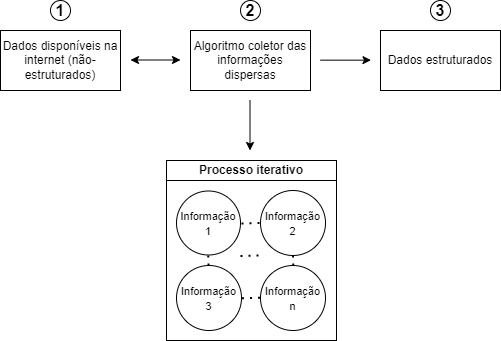
\includegraphics[scale = 0.85]{figuras/web_scraping_flow.png}
	\fonte{Elaboração do autor. Adaptado de \citeonline[p.~96]{hc_costa2016}}
\end{figure}

A maior parte dos dados disponíveis na internet possuem um arcabouço que não muda ao longo do tempo, apesar das informações contidas dentro do mesmo mudarem. O algoritmo de raspagem de dados \textit{web}, interagindo com os sites, localiza as informações, extrai os dados relevantes, estrutura e armazena os mesmos em formato painel, possibilitando futuras consultas.

Isto posto, a Figura \ref{figure:fluxo_web_scrap} nos permite observar o fluxo iterativo do coletor de dados, onde primeiro o algoritmo interpreta a esquematização da página \textit{web}. Por seguinte, iterativamente acessa o site, coletando as informações pré-definidas, extraindo os dados com base na disposição de como estão disponíveis. Essa dinâmica se repercute até que todos os dados foram coletados \cite{hc_costa2016}.

O uso desta técnica nos permite obter um grande volume de dados de forma estruturada, não só poupando tempo, como também permitindo a escalabilidade. Além disso, guarda as informações em um formato organizado, promovendo a reprodutibilidade, um princípio importante no método científico.

\subsubsection{Análise de sentimentos}

Diversas aplicações de análises de sentimento vem sendo desenvolvidas ao longo dos anos, levando em consideração que técnicas de mineração textual permitem a conversão de informações qualitativas em informações quantitativas estruturadas, facilitando a relação com pesquisas de cunho econômico, permitindo incorporá-las na modelagem econométrica. Como tratam \citeonline{liu2010sentiment_subjectivity}, a análise de sentimentos possui como principal objetivo definir técnicas automáticas para se extrair informações subjetivas de textos em linguagem natural para categorizar e identificar sentimentos em textos de forma estruturada para que possa ser utilizado por um sistema de apoio ou tomador de decisão.

A determinação do sentimento está intimamente relacionada ao formato como o texto é escrito, em que a partir de um conjunto de palavras, é possível estabelecer sua tonalidade. A maioria das abordagens de análises de sentimentos baseiam-se em dicionários léxicos, que são listas extensas de palavras que são categorizadas como positivas ou negativas de acordo com sua orientação semântica \cite{liu2010sentiment_subjectivity}.

A criação e validação dessas listas de palavras pode-se definir como um dos métodos mais robustos e confiáveis para a geração de dicionários léxicos, entretanto também é uma das maneiras que mais requisitam tempo. Dessa forma, diversas pesquisas aplicadas no tocante de análise de sentimentos baseia-se em dicionários léxicos previamente criados \cite{hutto2014vader}.

Um dos dicionários léxicos mais antigos criado foi introduzido por \citeonline{stone_etal1966}, denominado \textit{General Inquirer}, onde foi escrito manualmente. Foi desenvolvido como ferramenta para \textit{análise de conteúdo}, técnica usada por cientistas sociais, cientistas políticos e psicólogos para identificação objetiva de características específicas de mensagens. Dentre o total de palavras, 1915 categorizam-se como positivas e 2291 categorizam-se como negativas \cite{hutto2014vader}.

Ainda, tem-se que a semântica de um documento de texto é de extrema importância para sua análise, onde existem diversas técnicas para se lidar com a questão da semântica, podendo ser citadas a remoção de \textit{stopwords} e remoção de palavras e caracteres sem relevância. Muitos tipos de palavras não agregam de forma pertinente para o sentido de um documento textual, como preposições e conjunções, aparecendo repetidamente diversas vezes, podendo prejudicar o algoritmos de processamento de textos. Essas palavras são chamadas de \textit{stopwords} e, na etapa de limpeza dos dados, elas são removidas.

\subsubsubsection{A estatística tf-idf (term frequency-inverse document frequency)}

Uma das maneiras costumeiras de representar-se um texto é dividi-lo em \textit{tokens}, isto é, em palavras e outros elementos que deseja-se mapear no processamento de um documento. Conforme enunciam \citeonline{salton1975document_indexing}, entende-se que um documento é um conjunto de termos indexados que podem possuir pesos a partir da importância desse termo no documento, sendo assim pode-se representar Um documento como um vetor de $n$ dimensões como:

\begin{ceqn}
\begin{align} \label{eq:document_to_corpus}
D_{i} = (d_{i1}, d_{i2},...,d_{in})
\end{align}
\end{ceqn} em que $D_{in}$ representa o peso do $n$-ésimo termo. Sendo assim, tem-se que um \textit{Corpus} de documentos é um conjunto de documentos dispostos em um espaço vetorial, isto é, como se fosse um documento de documentos.

O método da estatística de \textit{term frequency-inverse document frequency} (tf-idf) consiste em considerar que a frequência dos \textit{tokens} de determinado documento importa para a elaboração da análise. 

A frequência de determinado termo em um documento é obtido através da quantidade de vezes que o termo surge, onde transforma-se cada documento em uma matriz de tuplas, sendo o primeiro elemento um determinado termo e o segundo elemento a frequência desse mesmo termo no documento. Para se ajustar a frequência dos termos no \textit{Corpus}, conforme apontam \citeonline{rajaraman2011mining}, é interessante considerar a proporcionalidade das frequências em relação ao tamanho do documento, tem-se então:

\begin{ceqn}
\begin{align} \label{eq:tf}
{tf}_{ij} = \frac{f_{ij}}{max_{k}f_{kj}}
\end{align}
\end{ceqn} onde $tf$ é a frequência do termo; $i$ é um termo em determinado documento $j$; e $k$ é o termo com maior frequência no documento. Ainda conforme \citeonline{rajaraman2011mining}, tem-se:

\begin{ceqn}
\begin{align} \label{eq:idf}
{idf}_{i} = \ln \left( \frac{N}{n_{i}} \right)
\end{align}
\end{ceqn} em que ${idf}_{i}$ é a frequência inversa de um termo $i$ que aparece $n$ vezes em $N$ documentos. Multiplicando a Equação \eqref{eq:tf} pela Equação \eqref{eq:idf}, chega-se então na estatística tf-idf de um termo $i$ em um documento $j$.

Em busca de considerar a influência de termos que são menos frequentes em um documento, entretando podem ser relevantes para a análise, calcula-se a frequência inversa do termo em determinado documento, minimizando a importância de palavras muito comuns e aumentando a importância de palavras mais raras. 

\subsection{Modelagem econométrica}

Nesta Subseção serão apresentados os processos da modelagem econométrica. Primeiramente é discursado sobre processos estocásticos e estacionariedade, apresentando os devidos testes, seguido pela apresentação do modelo VAR, que possibilita tanto verificar a causalidade de Granger, como elaborar a IRF. Após isso, são feitos testes de diagnóstico acerca de correlação serial e heterocedasticidade. Por fim, é apresentada a base de dados das atas do Copom e das variáveis macroeconômicas utilizadas na elaboração desta pesquisa.

\subsubsection{Processos aleatórios e séries estacionárias}

Conforme enunciado em \citeonline{gujarati_ecn2011}, define-se um processo aleatório como uma coleção de variáveis estocásticas ordenadas no tempo. Sendo assim, sugere-se que dados macroeconômicos, genericamente, são categorizados como processos aleatórios (denominados também como séries temporais). Da mesma maneira que se utiliza amostras de dados para efetuar inferências sobre uma determinada população, no campo de séries temporais, utiliza-se a realização do processo estocástico em questão para extrações inferenciais \cite{gujarati_ecn2011}.

De modo geral, caso a série temporal se enquadrar como estacionária, sua média e sua variância deverão ser constantes ao longo do tempo. Além disso, o valor da covariância entre dois períodos de tempo deverá depender somente da defasagem entre eles; de outro modo, a série não será estacionária. Tal processo estocástico é conhecido na literatura como fracamente estacionário \cite{gujarati_ecn2011, morettin2017estatistica}.

A partir de um modelo generalizado, pode-se representar diversas séries temporais e suas características. Sendo $Y_{t}$ um processo estocástico fracamente estacionário, como segue:

\begin{ceqn}
\begin{align} \label{eq:ts_generic_model}
 Y_{t} = \beta_{0} + \beta_{1} t + \beta_{2} Y_{t-1} + \mu_{t}
\end{align}
\end{ceqn} tem-se que $\beta_{0}$ é o coeficiente constante (de intercepto); $\beta_{1}$ é o coeficiente relacionado à medição do tempo $t$ (de tendência); $\beta_{2}$ é o coeficiente do termo autorregressivo (AR), que é a série no período anterior ($t-1$); e $\mu_{t}$ é um termo de erro do tipo ruído branco, a parte que o modelo não consegue captar \cite{gujarati_ecn2011}.

A depender dos valores obtidos para os estimadores de $\beta_{k}$, pode ser que a série temporal possua características de estacionariedade ou não. Supondo que $\mu_{t}$ seja um termo de erro do tipo ruído branco, com média igual à zero e variância $\sigma^2$ (constante); tem-se então que a série $Y_{t}$ é um passeio aleatório puro (sem deslocamento), conforme:

\begin{ceqn}
\begin{align} \label{eq:random_walk}
 Y_{t} = Y_{t-1} + \mu_{t}
\end{align}
\end{ceqn} em que $\beta_{0} = \beta_{1} = 0$ e $\beta_{2} = 1$. Constata-se que a variância da Equação \eqref{eq:random_walk} crescerá indefinitivamente conforme o aumento do tempo $t$, uma vez que $var(Y_{t}) = \sigma^2 t$, violando assim uma das condições de estacionariedade fraca \cite{gujarati_ecn2011}.

Subtraindo $Y_{t-1}$ de ambos os lados da Equação \eqref{eq:random_walk}, chega-se em:

\begin{ceqn}
\begin{align} \label{eq:rw_diff}
(Y_{t} - Y_{t-1}) = (Y_{t-1} - Y_{t-1}) + \mu_{t} \notag \\
(Y_{t} - Y_{t-1}) = \mu_{t} \notag \\
\Delta Y_{t} = \mu_{t}
\end{align}
\end{ceqn} onde $\Delta$ é chamado de operador de diferença, isto é, o valor da série no tempo $t$ subtraído do valor da série no tempo $t-1$. Assim como demonstrado por \citeonline{gujarati_ecn2011}, as primeiras diferenças de séries temporais de um passeio aleatório são estacionárias, e neste caso, são integradas de ordem 1, podendo ser representadas por $I(1)$, ou genéricamente como integradas de ordem $d \rightarrow I(d)$.

\subsubsubsection{Teste de raiz unitária de Dickey-Fuller Aumentado (ADF)}

Em modelos de séries temporais, a unidade de raiz é uma importante característica dos processos de realização da série que, caso não for adequadamente tratada, pode causar problemas de inferência. Reescrevendo a Equação \eqref{eq:random_walk} como:

\begin{ceqn}
\begin{align} \label{eq:rw_rho}
 Y_{t} = \rho Y_{t-1} + \mu_{t} \qquad (-1 \leq \rho \leq 1)
\end{align}
\end{ceqn} tem-se $\mu_{t}$ como termo de erro ruído branco; e $\rho$ como coeficiente de autocorrelação entre $Y_{t}$ e $Y_{t-1}$. Caso $\rho = 1$, a Equação \eqref{eq:rw_rho} será um processo de passeio aleatório e se terá problema de raiz unitária, ou seja, problema de estacionariedade na série. Subtraindo $Y_{t-1}$ de ambos os lados da Equação \eqref{eq:rw_rho} e aplicando o operador de diferença, é possível chegar em:

\begin{ceqn}
\begin{align} \label{eq:df_test}
Y_{t} - Y_{t-1} = \rho Y_{t-1} - Y_{t-1} + \mu_{t} \notag \\
\Delta Y_{t} = (\rho - 1) Y_{t-1} + \mu_{t} \notag \\
\Delta Y_{t} = \delta Y_{t-1} + \mu_{t}
\end{align}
\end{ceqn} em que $\delta = (\rho - 1)$.

Para se efetuar o teste de raiz unitária, deve-se estimar os parâmetros da Equação \eqref{eq:df_test}, testando a hipótese nula ($H_{0})$) contra a hipótese alternativa ($H_{1}$), como segue:

\begin{ceqn}
\begin{align} \label{eq:hipoteses_estacionariedade}
&H_{0}: \delta = 0 \\ % \qquad \rightarrow \text{série não estacionária}
&H_{1}: \delta < 0 %\qquad \rightarrow \text{série estacionária}
\end{align}
\end{ceqn}

Caso o resultado do teste for $\delta = 0$, terá-se então um $\rho = 1$, isto é, raiz unitária. Dessa forma, o processo estócastico testado trata-se de uma série não estacionária. Como demonstrado por \citeonline{UR_dickey_fuller1979} e abordado em \citeonline{gujarati_ecn2011}, o valor estimado de $t$ para o coeficiente $Y_{t-1}$ da Equação \eqref{eq:df_test} segue a estatística $\tau$ (tau). Os valores fundamentais da estatística $\tau$ foram computadas a partir de simulações de Monte Carlo, onde o teste ficou conhecido como teste de Dickey-Fuller. Com o objetivo de englobar diversas possibilidades, a estimação do teste é feito de três formas:

\begin{ceqn}
\begin{align} \label{eq:df_equations}
&\Delta Y_{t} = \delta Y_{t-1} + \mu_{t} \qquad \qquad \qquad \qquad \qquad \qquad \qquad \text{\textbf{(passeio aleatório)}} \\
&\Delta Y_{t} = \beta_{0} + \delta Y_{t-1} + \mu_{t} \qquad \qquad \qquad \text{\textbf{(passeio aleatório com deslocamento)}} \\
&\Delta Y_{t} = \beta_{0} + \beta_{1} t + \delta Y_{t-1} + \mu_{t} \quad \text{\textbf{(passeio aleatório com deslocamento e tendência)}} 
\end{align}
\end{ceqn}

A estatística tau calculada ($\tau_{calculada}$) pode ser obtida ao dividir o delta estimado ($\hat{\delta}$) pelo seu desvio-padrão ($\sigma_{\hat{\delta}}$), e caso seu módulo for maior do que o módulo da estatística tau crítica (|$\tau_{critica}$|), se rejeita a hipótese nula ($H_{0}$) de que não há estacionariedade, caso contrário, trata-se de uma série estacionária.

Para as situações em que os resíduos da série temporal ($\mu_{t}$) são correlacionados, ou seja, problema de autocorrelação, utiliza-se do teste de Dickey-Fuller Aumentado (ADF), em que trata de adicionar valores defasados da variável $Y_{t}$ na estimação, chegando-se na seguinte equação:

\begin{ceqn}
\begin{align} \label{eq:adf_equation}
\Delta Y_{t} = \beta_{0} + \beta_{1} t + \delta Y_{t-1} + \sum_{p=1}^{n}{\alpha_{p} \Delta Y_{t-p}} + \epsilon_{t}
\end{align}
\end{ceqn} em que $\epsilon_{t}$ é um termo de ruído branco e $p_{1,...,n}$ refere-se ao número de defasagens. 

O objetivo é adicionar termos suficientes na Equação \eqref{eq:adf_equation} de maneira que o erro $\epsilon_{t}$ seja serialmente não correlacionado, para que seja possível obter-se uma estimativa não viesada de $\delta$, que é o coeficiente defasado de $Y_{t-1}$. Embora haver mais parâmetros no teste de Dickey-Fuller Aumentado, ainda é testado se $\delta = 0$, seguindo a mesma distribuição assintótica da estatística de Dickey-Fuller, de forma que os mesmos valores de $\tau$ podem ser utilizados \cite{gujarati_ecn2011}.

Dada determinada ordem de defasagem máxima ($\rho_{maxima}$), a partir do critério de informação de Akaike (AIC) ou critério Bayesiano de Schwarz (BIC), pode-se selecionar a melhor extensão de defasagens para o modelo. Conforme apresentado em \citeonline{bueno2008}, a escolha do número máximo máximo de extensões dá-se pelo número inteiro obtido atráves de:

\begin{ceqn}
\begin{align} \label{eq:rho_max}
\rho_{maxima} = 12 \left(\frac{N}{100}\right)^\frac{1}{4}
\end{align}
\end{ceqn} em que $N$ é o tamanho da amostra. Dado um nível de significância ($\alpha$) de $5,00$\%, exibe-se na Tabela \ref{table:tabela_tau} os valores críticos para a estatística $\tau$.

\begin{table}[hbtp]
	\centering
	\caption{Valores críticos para a estatística $\tau$ dado um $\alpha = 5,00$\%} \label{table:tabela_tau}
	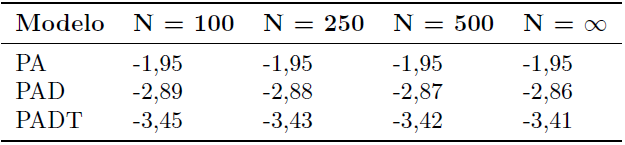
\includegraphics[scale = 0.75]{figuras/tabela_tau.PNG}
	\fonte{Elaboração do autor. Adaptado de \citeonline{fuller1976}.} 
\end{table}

Como ponto de observação, na primeira coluna, PA refere-se à passeio aleatório (sem constante), PAD refere-se à passeio aleatório com deslocamento (com constante) e PADT refere-se à passeio aleatório com deslocamento e tendência (com constante e tendência).

\subsubsubsection{Teste de raiz unitária de Phillips-Perron (PP)}

Outro teste conhecido é o teste desenvolvido por \citeonline{UR_phillips_perron1988}, em que propõem um método alternativo e não-paramétrico de controlar a autocorrelação ao testar-se a raiz unitária, permitindo que seja consistente mesmo havendo variáveis dependentes defasadas e correlação serial nos resíduos. Sendo assim, o teste de Phillips-Perron (PP) faz com que seja desnecessária a especificação de um modelo com ordem suficientemente autorregressivo para a eliminação do problema de autocorrelação \cite{bueno2008}.

Considerando a seguinte alternativa de regressão $\Delta Y_{t}$ e a sua respectiva estatística $Z_{t}$ associada, tem-se:

\begin{ceqn}
\begin{align} \label{eq:pp_1}
%&\Delta Y_{t} = \alpha Y_{t-1} + \mu_{t} \qquad \qquad \qquad \rightarrow Z_{t} \nonumber \\
\Delta Y_{t} = \omega + \alpha Y_{t-1} + \mu_{t} \qquad \rightarrow \qquad Z_{t, \omega} 
%&\Delta Y_{t} = \omega + \delta t + \alpha Y_{t-1} + \mu_{t} \qquad \rightarrow Z_{t, \tau} \nonumber
\end{align}
\end{ceqn} em que $\Delta$ é o operador da diferença e $\mu_{t}$ é um processo estacionário. Estima-se então o parâmetro $\hat{\alpha}$ de interesse:

\begin{ceqn}
\begin{align} \label{eq:pp_alpha}
\hat{\alpha} = \frac{\sum_{t=1}^{N}{(Y_{t-1} - \overline{Y}_{-1}) (Y_{t} - \overline{Y})}}{\sum_{t=1}^{N}{(Y_{t-1} - \overline{Y}_{-1})^2}} - 1
\end{align}
\end{ceqn} onde $\overline{Y}$ representa a média, sendo possível estimar a variância populacional $\hat{\sigma}^2$:

\begin{ceqn}
\begin{align} \label{eq:pp_sigma}
\hat{\sigma}^2 = \frac{\sum_{t=1}^{N}{(\Delta Y_{t} - \hat{\omega} - \hat{\alpha} Y_{t-1})^2}}{N}
\end{align}
\end{ceqn} e a partir da Equação \eqref{eq:pp_sigma} pode-se calcular a variância de longo prazo $\hat{\upsilon}^2$:

\begin{ceqn}
\begin{align} \label{eq:pp_vega}
\hat{\upsilon}^2 = \hat{\sigma}^2 + \frac{2}{N} \sum_{j=1}^{M}{\phi \left(\frac{j}{M+1} \right)} \sum_{t=j+1}^{N}{\hat{\mu}_{t} \hat{\mu}_{t-j}}
\end{align}
\end{ceqn} podendo-se chegar afinal na estatística de PP, dada por:

\begin{ceqn}
\begin{align} \label{eq:pp_total}
\hat{Z}_{t, \omega} = \hat{\tau}_{\omega} \left(\frac{\hat{\sigma}}{\hat{\upsilon}} \right) - \frac{1}{2} \left(\frac{\hat{\upsilon}^2 - \hat{\sigma}^2}{\hat{\upsilon} \sqrt{N^{-2} \sum_{t=1}^{N} Y_{t-1}^2}} \right)
\end{align}
\end{ceqn} em que na variância de longo prazo estão inclusas todas as autocovariâncias do processo $\mu_{t}$.

A interpretação do teste de PP é a mesma do que a do teste de ADF, uma vez que possuem a mesma distribuição assintótica, tendo-se que a hipótese nula ($H_{0}$) é de que a série apresenta raiz unitária contra a hipótese alternativa ($H_{1}$) de que a série é estacionária \cite{bueno2008, gujarati_ecn2011}.

\subsubsubsection{Teste de raiz unitária de Kwiatkowski–Phillips–Schmidt–Shin (KPSS)}

Devido à facilidade de implementação e bom funcionamento dos testes de raiz unitária ADF e PP, eles são popularmente utilizados. Entretanto, tanto o teste ADF quanto o teste de PP possuem como $H_{0}$ a presença de raiz unitária, isto é, a não estacionariedade. De qualquer maneira, a literatura acerca do tema frequentemente aceita a $H_{1}$, caso inexistam evidências contrárias a $H_{0}$, ainda mais quando trata-se de séries macroeconômicas. Devido a esse fator, faz-se de bom uso a aplicação de um teste que tenha como $H_{0}$ a estacionariedade e outro que a tenha como $H_{1}$ \cite{kennedy2008guide_to_econometrics}.

O teste desenvolvido por \citeonline{UR_kpss1992}, conhecido como teste KPSS (mnemônico dos autores), possui a estacionariedade da série como hipótese nula ($H_{0}$), frente a não estacionariedade como hipótese alternativa ($H_{1}$), como segue:

\begin{ceqn}
\begin{align} \label{eq:hipoteses_kpss}
&H_{0}: Y_{t} \thicksim I(0) \\
&H_{1}: Y_{t} \thicksim I(1) 
\end{align}
\end{ceqn}

O objetivo é usar o teste como complementar aos testes tradicionais, distinguindo assim a raiz unitária de séries cujos dados não são suficientemente conclusivos (como séries macroeconômicas), caracterizando-se assim mais assertivamente a série \cite{bueno2008}.

O teste KPSS decompõe a série em questão em três partes, conforme:

\begin{ceqn}
\begin{align} \label{eq:kpps_ts_1}
Y_{t} = \eta t + \phi_{t} + \epsilon_{t}
\end{align}
\end{ceqn} onde $\eta t$ é o elemento de tendência determinística, $\phi_{t}$ é o elemento de passeio aleatório e $\epsilon_{t}$ é o elemento de erro estacionário. É efetuado então um processo de soma parcial dos resíduos, como:

\begin{ceqn}
\begin{align} \label{eq:kpps_ts_2}
S_{t} = \sum_{t=1}^{N}{\hat{e}_{t}}
\end{align}
\end{ceqn} no qual $\hat{e}_{t}$ são os erros da Equação \eqref{eq:kpps_ts_1}. Tendo a variância de longo prazo ($\hat{\upsilon}^2$) como definida na Equação \eqref{eq:pp_sigma}, chega-se à estatística do teste KPSS, dada por:

\begin{ceqn}
\begin{align} \label{eq:stat_kpss}
KPSS = \sum_{t=1}^{N}{\frac{S_{t}^2}{N^2 \hat{\upsilon}^2}}
\end{align}
\end{ceqn}

Caso $Y_{t}$ for um processo estacionário, então $S_{t} \thicksim I(1)$ e o numerador da estatística KPSS será um estimador da variância de $S_{t}$, tendo assim um limite assintótico. Já o denominador observado na Equação \eqref{eq:stat_kpss} assegura que a distribuição seja livre de ruídos. Na outra mão, caso $Y_{t} \thicksim I(1)$, o numerador crescerá ilimitadamente, fazendo a estatística KPSS ficar muito elevada.  \cite{bueno2008}.

Compara-se então a estatística calculada com os valores críticos a determinado nível de significância, sendo que se o valor calculado for maior que o valor crítico, rejeita-se a $H_{0}$ de estacionariedade. Os valores críticos para a realização do teste de KPSS, que foram calculados e apresentados em \citeonline{UR_kpss1992}, são utilizados como parâmetros de comparação.

Já em relação a ordem de defasagem máxima ($\rho_{maxima}$) na regressão, como apontado em \citeonline{tseries2022R_package}, será utilizado o número inteiro obtido através de:

\begin{ceqn}
\begin{align} \label{eq:rho_max_kpss}
\rho_{maxima} = 4 \left( \frac{N}{100} \right)^\frac{1}{4}
\end{align}
\end{ceqn} alternativamente à Equação \eqref{eq:rho_max}.

\subsubsection{Vetores autorregressivos (VAR)}

A modelagem econômica em geral é caracterizada por haver diversas variáveis, sendo assim, modelos univariados são limitados para expressar modelos econômicos. O VAR permite que sejam expressos modelos econômicos e se estimem seus parâmetros. Genericamente falando, pode-se definir um modelo autorregressivo de ordem $p$, isto é, um VAR($p$) como:

\begin{ceqn}
\begin{align} \label{eq:var_1}
A Y_{t} = B_{0} + \sum_{i=1}^{p}{B_{i} Y_{t-i}} + \epsilon_{t}
\end{align}
\end{ceqn} onde $A$ representa uma matriz $n \times n$ que define as restrições contemporâneas; $Y_{t}$ é um vetor $n \times 1$ das variáveis endógenas no período $t$; $B_{0}$ é um vetor de constantes $n \times 1$; $B_{i}$ é uma matriz $n \times n$ dos parâmetros referentes ao vetor $Y_{t-i}$, que são as variáveis endógenas defasadas $i$ vezes, possuindo dimensão $n \times 1$; e por fim $\epsilon_{t}$ é um vetor $n \times 1$ de erros do tipo ruído branco \cite{bueno2008}.

A Equação \eqref{eq:var_1} demonstra as relações entre as variáveis endógenas em sua forma estrutural, onde os choques $\epsilon_{t}$ são chamados de choques estruturais, uma vez que afetam de forma individual cada uma das variáveis endógenas. Por causa disso, o modelo costumeiramente é estimado na sua forma reduzida, multiplicando a equação por $A^{-1}$, conforme:

\begin{ceqn}
\begin{align} \label{eq:var_2}
Y_{t} = A^{-1} B_{0} + \sum_{i=1}^{p}{A^{-1} B_{i} Y_{t-i}} + A^{-1} \epsilon_{t}
\end{align}
\end{ceqn} onde $C \equiv A^{-1} B_{0}$; $\phi_{i} \equiv A^{-1} B_{i}$ e $e_{t} \equiv A^{-1} \epsilon_{t}$, chegando-se então em:

\begin{ceqn}
\begin{align} \label{eq:var_3}
Y_{t} = C + \sum_{i=1}^{p}{\phi_{i} Y_{t-i}} + e_{t}
\end{align}
\end{ceqn}

Convenientemente, conforme \citeonline{enders2008econometrics}, será considerado o modelo disposto na Equação \eqref{eq:var_3} como um modelo bivariado com defasagem de ordem igual a 1, chegando no sistema:

\begin{ceqn}
\begin{align} \label{eq:var_4}
&y_{t} = b_{10} - a_{12} z_{t} + b_{11} y_{t-1} + b_{12} z_{t-1} + \sigma_{y} \epsilon_{yt} \\
&z_{t} = b_{20} - a_{21} y_{t} + b_{21} y_{t-1} + b_{22} z_{t-1} + \sigma_{z} \epsilon_{zt}
\end{align}
\end{ceqn}

Nota-se que as variáveis são mutuamente influenciadas umas pelas outras, tanto com seus valores atuais quanto com seus valores defasados. O VAR não pode ser diretamente estimado, considerando que as variáveis atuais $z_{t}$ e $y_{t}$ são isoladamentes correlacionadas aos erros $\epsilon_{yt}$ e $\epsilon_{zt}$, respectivamente. Isso acontece, pois cada uma dessas variáveis depende do comportamento da outra, tendo como objetivo do VAR encontrar a trajetória da variável de interesse a partir da efetuação de um choque nesses erros \cite{bueno2008}.

\subsubsubsection{Causalidade de Granger}

A causalidade no sentido de Granger acontece quando uma variável é capaz de prever outra variável e em sob quais condições, isto é, quando é possível utilizar uma variável, seja defasada ou não, para prever outra variável em determinado período de tempo. O objetivo é determinar se $y$ ajuda a prever $z$ e caso isso não aconteça, tem-se que $y$ não Granger-causa $z$. O teste feito então é:

\begin{ceqn}
\begin{align} \label{eq:granger_causality}
z_{t} = \phi_{20} + \sum_{i=1}^{p}{\phi_{i, 21} y_{t-i}} + \sum_{i=1}^{p}{\phi_{i, 22} z_{t-i}} + e_{2t}
\end{align}
\end{ceqn} onde a seguinte hipótese nula ($H_{0}$) é testada frente a hipótese alternativa ($H_{1}$):

\begin{ceqn}
\begin{align} \label{eq:granger_causality_hip}
&H_{0}: \phi_{i, 21} = 0 \qquad \text{(ausência de Granger-causalidade)}\\
&H_{1}: \phi_{i, 21} \neq 0 \qquad \text{(presença de Granger-causalidade)}
\end{align}
\end{ceqn} em que a estatística do teste ($S_{1}$) é dada por:

\begin{ceqn}
\begin{align} \label{eq:granger_causality_stat}
S_{1} = \frac{\frac{(e_{\gamma}^2 - e_{\mu}^2)}{p}}{\frac{e_{\mu}^2}{N - 2p - 1}} \qquad \rightarrow \qquad F(p; N - 2p - 1)
\end{align}
\end{ceqn} tal qual $\gamma$ representa restrito e $\mu$ representa irrestrito. 

Caso $S_{1} > F$ dado um nível de significância ($\alpha$), rejeita-se a hipótese nula de que $y$ não Granger-causa $z$, ou seja, se conclui que existe uma relação de causalidade no sentido de Granger \cite{bueno2008, gujarati_ecn2011}.

Para se definir a quantidade ideal de defasagens a serem inseridas dentro do sistema de equações, pode-se utilizar os critérios de informação, em que atribuem penalidade conforme aumenta-se o número de regressores, por impactar na soma dos resíduos do modelo. Estes critérios então minimizam uma função que baseia-se nos resíduos da regressão estimada, penalizada pela quantidade de regressores que foram utilizados \cite{bueno2008}.

O modelo mais ideal será o com maior parcimônia, isto é, com menor número de parâmetros, satisfazendo com que os resíduos sejam os menores possíveis. Geralmente, o critério de especificação possui o seguinte formato:

\begin{ceqn}
\begin{align} \label{eq:general_inf_crit}
CE = \ln \hat{\sigma}^2 (N) + c_{N} \varphi (N)
\end{align}
\end{ceqn} onde $\hat{\sigma}^2 (N) = \frac{\sum_{t=1}^{N}{\hat{\epsilon}_{t}^2}}{N} $ é a variância estimada dos resíduos; $c_{N}$ é o número de parâmetros estimados; e $\varphi (N)$ é a ordem do processo, que penaliza a falta de parcimoniosidade. Dessa forma, existem três principais critérios de informação, onde a estatística de Critério de Informação Bayesiano (BIC) se dá por:

\begin{ceqn}
\begin{align} \label{eq:BIC}
BIC(p,q) = \ln \hat{\sigma}^2 + n \frac{ln N}{N}
\end{align}
\end{ceqn} no qual $n = p + q$ caso o modelo não possuir constante ou $n = p + q + 1$ caso houver constante.

Outro critério é a estatística de Critério de Informação de Akaike (AIC), em que:

\begin{ceqn}
\begin{align} \label{eq:AIC}
AIC(p,q) = \ln \hat{\sigma}^2 + n \frac{2}{N}
\end{align}
\end{ceqn}

Por fim, a estatística Hannan-Quinn (HQ) é conforme segue:

\begin{ceqn}
\begin{align} \label{eq:HQ}
HQ(p,q) = \ln \hat{\sigma}^2 + n \frac{2}{N} \ln (\ln N)
\end{align}
\end{ceqn}

A primeira parte da Equação \eqref{eq:general_inf_crit} mede a adequação do processo, em que quanto menor a variância dos resíduos, melhor. Entretanto, uma redução de variância que foi obtida ao introduzir mais parâmetros é penalizada pela segunda parte da equação. Dessa maneira, deseja-se o menor AIC, BIC ou HQ possível \cite{bueno2008}.

\subsubsubsection{Função de impulso-resposta (IRF)}

Assim como existe a possibilidade de se retratar um modelo autorregressivo como seu componente de média móvel, pode-se representar um modelo VAR($p$) como um Vetor de Média Móvel (VMA), isto é, um VMA($\infty$). Dessa forma, como abordado em \citeonline{sims1980macroeconomics}, elabora-se projeções distintas a partir da efetuação de choques nas variáveis introduzidas no modelo VAR($p$). Considerando uma abordagem matricial para um modelo de VAR($1$), tem-se:

\begin{ceqn}
\begin{align} \label{eq:mat_var}
\begin{bmatrix}
y_{1t} \\
y_{2t}
\end{bmatrix}
=
\begin{bmatrix}
\alpha_{1} \\
\alpha_{2}
\end{bmatrix}
+
\begin{bmatrix}
\phi_{11} y_{1, t-1} \\
\phi_{12} y_{1, t-1}
\end{bmatrix}
+
\begin{bmatrix}
\phi_{21} y_{2, t-1} \\
\phi_{22} y_{2, t-1}
\end{bmatrix}
+
\begin{bmatrix}
\mu_{1t} \\
\mu_{2t}
\end{bmatrix}
\end{align}
\end{ceqn} no qual, reescrevendo a Equação \eqref{eq:mat_var}, chega-se em:

\begin{ceqn}
\begin{align} \label{eq:mat_var_2}
\begin{bmatrix}
y_{1t} \\
y_{2t}
\end{bmatrix}
=
\begin{bmatrix}
\overline{y}_{1} \\
\overline{y}_{2}
\end{bmatrix}
+
\sum_{i=0}^{\infty}{\begin{bmatrix} \phi_{11} & \phi_{12} \\ \phi_{21} & \phi_{22} \end{bmatrix}^i}
\begin{bmatrix}
\mu_{1, t-i} \\
\mu_{2, t-i}
\end{bmatrix}
\end{align}
\end{ceqn} em que a Equação \eqref{eq:mat_var_2} representa $\begin{bmatrix} y_{1t} \\ y_{2t} \end{bmatrix}$ em termos de $\begin{bmatrix} \mu_{1t} \\ \mu_{2t} \end{bmatrix}$. Entretranto, reescrevendo em relação a $\begin{bmatrix} \mu_{y_{1}t} \\ \mu_{y_{2}t} \end{bmatrix}$, conforme aborda \citeonline{enders2008econometrics}, obtém-se:

\begin{ceqn}
\begin{align} \label{eq:mat_var_3}
\begin{bmatrix}
\mu_{1t} \\
\mu_{2t}
\end{bmatrix}
=
\frac{1}{1-b_{12}b_{21}} \begin{bmatrix} 1 & -b_{12} \\ -b_{21} & 1 \end{bmatrix}
\begin{bmatrix}
\mu_{y_{1}t} \\
\mu_{y_{2}t}
\end{bmatrix}
\end{align}
\end{ceqn} onde ao combinar a Equação \eqref{eq:mat_var_2} e a Equação \eqref{eq:mat_var_3}, terá-se:

\begin{ceqn}
\begin{align} \label{eq:mat_var_4}
\begin{bmatrix}
y_{1t} \\
y_{2t}
\end{bmatrix}
=
\begin{bmatrix}
\overline{y}_{1} \\
\overline{y}_{2}
\end{bmatrix}
+
\frac{1}{1-b_{12}b_{21}}
\sum_{i=0}^{\infty}{\begin{bmatrix} \phi_{11} & \phi_{12} \\ \phi_{21} & \phi_{22} \end{bmatrix}^i}
\begin{bmatrix} 1 & -b_{12} \\ -b_{21} & 1 \end{bmatrix}
\begin{bmatrix}
\mu_{y_{1}t} \\
\mu_{y_{2}t}
\end{bmatrix}
\end{align}
\end{ceqn} em que, para simplificar, define-se a matriz $\Theta_{i}$ como:

\begin{ceqn}
\begin{align} \label{eq:irf}
\Theta_{i} = \frac{A_{1}^i}{1-b_{12}b_{21}} \begin{bmatrix} 1 & -b_{12} \\ -b_{21} & 1 \end{bmatrix}
\end{align}
\end{ceqn} e com isso, a representação de média móvel introduzida na Equação \eqref{eq:mat_var_2} pode ser reescrita conforme:

\begin{ceqn}
\begin{align} \label{eq:irf_2}
\begin{bmatrix}
y_{1t} \\
y_{2t}
\end{bmatrix}
=
\begin{bmatrix}
\overline{y}_{1} \\
\overline{y}_{2}
\end{bmatrix}
+
\sum_{i=0}^{\infty}{\begin{bmatrix} \Theta_{11}(i) & \Theta_{12}(i) \\ \Theta_{21}(i) & \Theta_{22}(i) \end{bmatrix}^i}
\begin{bmatrix}
\mu_{y_{1}t} \\
\mu_{y_{2}t}
\end{bmatrix}
\end{align}
\end{ceqn} sendo assim, de maneira mais compacta:

\begin{ceqn}
\begin{align} \label{eq:irf_3}
Y_{t} = \overline{Y}_{t} + \sum_{i=0}^{\infty}{\Theta_{i} \mu_{t-i}}
\end{align}
\end{ceqn} em que os elementos da matriz $\Theta_{i}$ são denominados multiplicadores de impacto de um choque sobre as variáveis endógenas. Dessa forma, o impacto total de um choque de $\mu_{y_{1}t}$ sobre $Yt_{t+n}$ é dado por $\sum_{i=0}^{n}{\Theta_{11}(i)}$, sendo que caso $y_{1}$ e $y_{2}$ forem estacionárias, os valores de $\Theta_{xz}(i)$ convirjirão para zero conforme aumentar-se $i$, implicando que os choques não possuem efeitos permanentes em séries estacionárias \cite{bueno2008}.

\subsubsection{Autocorrelação serial}

Define-se autocorrelação serial como a correlação entre o termo de erro $\mu$ em determinado período $t$ e o termo de erro $\mu$ em seu período anterior $t-1$, isto é, a relação de $\mu_{t}$ e $\mu_{t-1}$. Levando em consideração uma série temporal na forma:

\begin{ceqn}
\begin{align} \label{eq:ts_autocorrel}
 Y_{t} = \beta_{0} + \beta_{1} X_{t} + \mu_{t}
\end{align}
\end{ceqn} supõe-se que o termo de erro $\mu_{t}$ é gerado pelo mecanismo:

\begin{ceqn}
\begin{align} \label{eq:ts_residual}
\mu_{t} = \lambda \mu_{t-1} + \epsilon_{t} \qquad (-1 < \lambda < 1)
\end{align}
\end{ceqn} em que $\lambda$ é o coeficiente de autocovariância e $\epsilon_{t}$ é o termo de erro estocástico, ao qual atende à hipótese padrão dos Mínimos Quadrados Ordinários (MQO):

\begin{ceqn}
\begin{align} \label{eq:ts_error_white_noise}
&E(\epsilon_{t}) = 0 \nonumber \\
&var(\epsilon_{t}) = \sigma^2 \\
&cov(\epsilon_{t}, \epsilon_{t+s}) = 0 \qquad (s \neq 0) \nonumber
\end{align}
\end{ceqn} sendo que por possuir tais propriedades, o termo de erro $\epsilon_{t}$ é denominado de ruído branco.

A Equação \eqref{eq:ts_residual} é conhecida como processo autorregressivo de primeira ordem de Markov e aponta que o valor do erro no período atual $t$ depende de uma proporção $\lambda$ do seu valor no período anterior, somado de um termo de erro totalmente aleatório $\epsilon_{t}$ \cite{gujarati_ecn2011}.

\subsubsubsection{Teste de Durbin-Watson (DW)}

Para verificação da existência - e se cabível o grau - de autocorrelação, um popular teste que é empregado é a estatística $d$ introduzida por \citeonline{durbin_watson1950}, definida como:

\begin{ceqn}
\begin{align} \label{eq:durbin_watson}
d = \frac{\sum{\hat{\mu}_{t}^2} + \sum{\hat{\mu}_{t-1}^2} - 2 \sum{\hat{\mu}_{t} \hat{\mu}_{t-1}}}{\sum{\hat{\mu}_{t}^2}} 
\end{align}
\end{ceqn} considerando que $\sum{\hat{\mu}_{t}^2} \approx \sum{\hat{\mu}_{t-1}^2}$, tem-se então:

\begin{ceqn}
\begin{align} \label{eq:durbin_watson_2}
d \approx 2 \left( 1 - \frac{\sum{\hat{\mu}_{t} \hat{\mu}_{t-1}}}{\sum{\hat{\mu}_{t}^2}} \right)
\end{align}
\end{ceqn} em que $\approx$ significa aproximadamente. Definindo:

\begin{ceqn}
\begin{align} \label{eq:dw_lambda}
\hat{\lambda} = \frac{\sum{\hat{\mu}_{t} \hat{\mu}_{t-1}}}{\sum{\hat{\mu}_{t}^2}}
\end{align}
\end{ceqn} pode-se expressar a Equação \eqref{eq:durbin_watson_2} como:

\begin{ceqn}
\begin{align} \label{eq:durbin_watson_3}
d \approx 2 (1 - \hat{\lambda})
\end{align}
\end{ceqn} onde $\hat{\lambda}$ é o coeficiente de covariância estimado da Equação \eqref{eq:ts_residual}.

Considerando que $-1 < \lambda < 1$, a Equação \eqref{eq:durbin_watson_3} denota que $0 \leq d \leq 4$. Valores próximos de zero para a estatística $d$ indicam correlação positiva, ficando próximo de 2 de acordo com menor evidência de autocorrelação. 

A Figura \ref{figure:intervalos_dw} apresenta as regras de decisão determinadas por \citeonline{durbin_watson1950}, em que $d_{L}$ denota o limite inferior da estatística $d$ e $d_{U}$ denota o limite superior da estatística $d$.

\begin{figure}[hbtp]
	\centering
	\caption{Zonas da estatística $d$ de Durbin-Watson} \label{figure:intervalos_dw}
	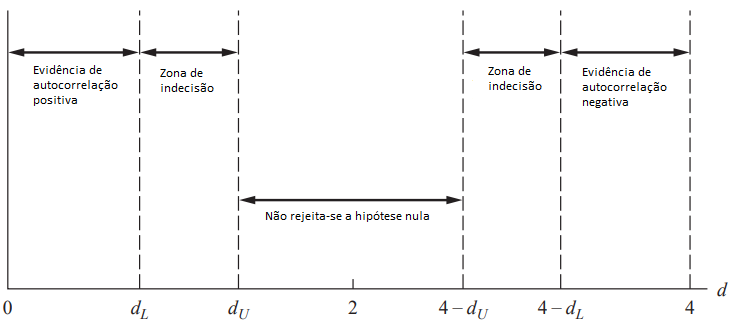
\includegraphics[scale = 0.65]{figuras/figura_durbin_watson.PNG}
	\fonte{Elaboração do autor. Adaptado de \citeonline{gujarati_ecn2011}.}
\end{figure}

É testado então a hipótese nula ($H_{0}$) contra a hipótese alternativa ($H_{1}$), tal qual:

\begin{ceqn}
\begin{align} \label{eq:hipoteses_autocorrelacao}
&H_{0}: \text{nenhuma autocorrelação, positiva ou negativa} \\
&H_{1}: \text{presença de autocorrelação}
\end{align}
\end{ceqn}

Salienta-se que $d_{L}$ e $d_{U}$ dependem do tamanho da amostra e da quantidade de variáveis explicativas do modelo; e caso $d_{U} < d < (4 - d_{U})$, não rejeita-se a hipótese nula ($H_{0}$) de ausência de autocorrelação serial \cite{gujarati_ecn2011}.

\subsubsubsection{Teste de Breusch-Godfrey (BG)}

Conforme apontado em \citeonline{gujarati_ecn2011}, para se evitar algumas armadilhas do teste $d$ de Durbin-Watson, \citeonline{breusch1978test} e \citeonline{godfrey1978test} desenvolveram um teste de autocorrelação que é genérico, não permitindo regressores não estocásticos (como valores defasados do regressando); esquemas autorregressivos de ordem superior; e médias móveis simples ou de ordem mais elevada de resíduos do tipo ruído branco, como $\epsilon_{t}$ na Equação \eqref{eq:ts_residual}.

O teste BG, também conhecido como teste do Multiplicador de Lagrange (LM), pressupõe que o termo de erro $\mu_{t}$ da Equação \eqref{eq:ts_autocorrel} siga um esquema autorregressivo de ordem $p$, como evidenciado em:

\begin{ceqn}
\begin{align} \label{eq:bg_1}
\mu_{t} = \lambda_{1} \mu_{t-1} + \lambda_{2} \mu_{t-2} + [...] + \lambda_{p} \mu_{t-p} + \epsilon_{t}
\end{align}
\end{ceqn} em que $\epsilon_{t}$ é um termo de erro do tipo ruído branco, tal qual apresentado em \eqref{eq:ts_error_white_noise}. O teste LM baseia-se em efetuar a regressão original, obtendo-se assim os resíduos estimados $\hat{\mu}_{t}$ e após isso introduzir os valores defasados dos resíduos como regressores adicionais no modelo:

\begin{ceqn}
\begin{align} \label{eq:bg_2}
\hat{\mu}_{t} = \alpha_{0} + \alpha_{1} X_{t} + \hat{\lambda}_{1} \hat{\mu}_{t-1} + \hat{\lambda}_{2} \hat{\mu}_{t-2} + [...] + \hat{\lambda}_{p} \hat{\mu}_{t-p} + \epsilon_{t}
\end{align}
\end{ceqn}

Tendo N como o tamanho da amostra e $R^2$ como o coeficiente de determinação da Equação \eqref{eq:bg_2}, \citeonline{breusch1978test} e \citeonline{godfrey1978test} demonstraram que para amostras grandes ($N \rightarrow \infty$), a relação $(N-p) R^2$ seguirá uma distribuição qui-quadrado com $p$ graus de liberdade, sendo assim:

\begin{ceqn}
\begin{align} \label{eq:chi_squared}
(N-p) R^2 \thicksim \chi_{p}^2
\end{align}
\end{ceqn}

Realiza-se então a testagem de hipóteses a determinado nível de significância ($\alpha$), tendo a hipótese nula ($H_{0}$) a ser testada como segue:

\begin{ceqn}
\begin{align} \label{eq:h0_bg_test}
H_{0}: \lambda_{1} = \lambda_{2} = [...] = \lambda_{p} = 0 \quad \rightarrow \quad \text{ausência de autocorrelação nos resíduos}
\end{align}
\end{ceqn}

Desse modo, caso $(N-p) R^2$ exceder o valor crítico ao nível determinado de $\alpha$, rejeita-se a $H_{0}$, em que pelo menos um dos $\lambda_{i}$ na Equação \eqref{eq:bg_2} é estatísticamente significantemente diferente de zero \cite{gujarati_ecn2011, bueno2008}.

O fato de uma série possuir autocorrelação faz com que a eficiência dos esimadores de MQO seja afetada, subestimando assim a variância - e por consequência, os erros padrão - do modelo. Contudo, estimadores MQO permanecem não tedenciosos, convergindo assim para seu valor populacional verdadeiro \cite{gujarati_ecn2011}.

\subsubsection{Heterocedasticidade da variância dos resíduos}

Não só autocorrelação serial é um problema, como os resíduos de determinada regressão podem ser heterocedásticos, isto é, sua variância não será constante ao longo do tempo (indiferentemente dos valores assumidos pela(s) variável(is) independente(s)). Os fatos de linearidade e parâmetros do modelo não serem tendenciosos não são alterados pela aparição de heterocedasticidade nas estimativas, apesar disso, caso tiver-se resíduos que forem heterocedásticos, terá-se perda de eficiência, uma vez que distorcem as variâncias do modelo e dos estimadores \cite{gujarati_ecn2011}.

Assim como é levantado em \citeonline{gujarati_ecn2011}, diversos testes de heterocedasticidade foram propostos com o decorrer dos anos, podendo ser citados o teste de \citeonline{park1966heterocedast}, o teste de \citeonline{glejser1969heterocedast}, o teste de \citeonline{goldfeld_quandt1972heterocedast}, o teste de \citeonline{breusch_pagan1979heterocedast} e o teste geral de \citeonline{white1980heterocedast}.

%\subsubsubsection{Teste geral de White}

%Entretanto, o teste mais popular é conhecido como o teste geral de heterocedasticidade de \citeonline{white1980heterocedast}, principalmente por causa de sua fácil implementação. Considerando um modelo do tipo:

%\begin{ceqn}
%\begin{align} \label{eq:ts_generic_white_heterocedast}
%Y_{t} = \beta_{1} + \beta_{2} X_{2t} + \beta_{3} X_{3t} + \mu_{t}
%\end{align}
%\end{ceqn} obtendo-se os resíduos $\hat{\mu}_{t}$. É feita então uma nova regressão, em que os resíduos ao quadrado da regressão feita na Equação \eqref{eq:ts_generic_white_heterocedast} são calculados contra as variáveis $X_{i, t}$ originais, seus valores ao quadrado e seus produtos cruzados:

%\begin{ceqn}
%\begin{align} \label{eq:ts_white}
%\hat{\mu}_{t}^2 = \alpha_{1} + \alpha_{2} X_{2t} + \alpha_{3} X_{3t} + \alpha_{4} X_{2t}^2 + \alpha_{5} X_{3t}^2  + \alpha_{6} X_{2t} X_{3t} + \epsilon_{t}
%\end{align}
%\end{ceqn} onde, podem ser incluídos também componentes com expoentes mais altos. Sob a hipótese nula ($H_{0}$) de que não há heterocedasticidade contra a hipótese alternativa ($H_{1}$) de que há:

%\begin{ceqn}
%\begin{align} \label{eq:white_hipoteses}
%&H_{0}: \alpha_{1} = \alpha_{2} = \alpha_{3} = [...] = \alpha_{n} = 0 \\
%&H_{1}: \text{pelo menos um dos } \alpha_{n} \neq 0
%\end{align}
%\end{ceqn} em que, obtendo-se o coeficiente de determinação ($R^2$) da Equação \eqref{eq:ts_white} e multiplicando-se pelo tamanho da amostra ($N$), chega-se na estatística do teste, que seguirá uma distribuição qui-quadrado com graus de liberdade ($gl$) igual ao número de parâmetros da regressão:

%\begin{ceqn}
%\begin{align} \label{eq:chi_squared_white}
%N R^2 \thicksim \chi_{gl}^2
%\end{align}
%\end{ceqn} sendo que caso a $\chi_{calculada}^2 > \chi_{critica}^2$ a determinado nível de $\alpha$, a conclusão é de que há heterocedasticidade, sendo assim rejeita-se a $H_{0}$ \cite{gujarati_ecn2011}.

%Destaca-se que, conforme apontado por \citeonline{gujarati_ecn2011}, mesmo havendo resíduos com variância heterocedástica, existe a possibilidade de se conseguir estimativas estatísticamente consistentes das variâncias dos estimadores, por meio dos erros padrão corrigidos pelo teste de heterocedasticidade de White.



%\subsection{Cointegração entre variáveis} \label{subsection:cointegracao}

%Dentro do ambiente econômico existe a possibilidade de se encontrar relações econométricas entre variáveis sem que efetivamente haja alguma relação de causa entre elas, isto é, uma regressão espúria (sem sentido). Para se confirmar caso os resultados foram alcançados de forma acidental, pode-se analisar a estacionariedade do resíduo $\mu_{t}$, e efetuar uma regressão nova com as variáveis em $I(1)$. Nesta situação, se $\mu_{t}$ for não estacionário, terá-se um caso de regressão sem sentido, sendo assim, o coeficiente de determinação $R^2$ não deverá ser elevado \cite{gujarati_ecn2011, bueno2008}.

%Define-se que duas variáveis são cointegradas caso elas tiverem uma relação de equilíbrio de longo prazo. Pode-se testar a existência de uma relação por meio do teste ADF nos resíduos de uma regressão qualquer, tal qual:

%\begin{ceqn}
%\begin{align} \label{eq:coint_generic_reg}
%Y_{t} = \beta_{0} + \beta_{1} X_{t} + \mu_{t}
%\end{align}
%\end{ceqn} onde $Y_{t} \thicksim I(1)$ e $X_{t} \thicksim I(1)$. Caso ambas as séries forem cointegradas, o resíduo $\mu_{t} \thicksim I(0)$, sendo que o $\beta_{1}$ será o parâmetro de cointegração. Entretanto, como $\hat{\mu}_{t}$ se baseia no $\hat{\beta}_{1}$, isto é, valores estimados, os valores tabelados do teste ADF não são apropriados \cite{gujarati_ecn2011}.

%\subsubsection{Teste de Engle-Granger}

%Pela razão dos valores tabelados do teste ADF são serem apropriados para se concluir a relevância estatística, foi-se calculado e tabelado novos valores para a conclusão do teste, conhecido como teste de \citeonline{engle_granger1987}. Será denominado teste Aumentado de Engle e Granger caso forem incluídas defasagens de $Y_{t}$ \cite{gujarati_ecn2011, bueno2008}.

%Conforme elucida \citeonline{bueno2008}, em busca de maior robustez estatística, novos valores críticos foram calculados para o $\tau$ de Engle e Granger, levando o tamanho da amostra $N$ em consideração, desenvolvido por \citeonline{mackinnon2010critical}:

%\begin{ceqn}
%\begin{align} \label{eq:mackinnon_crit_values}
%\tau = \gamma_{0} + \gamma_{1} N + \gamma_{2} N^2
%\end{align}
%\end{ceqn} em que $\gamma_{i}$ são os parâmetros tabelados.

%\subsubsection{Teste de Johansen}

%Outro teste de cointegração é o proposto por \citeonline{johansen1991}

%\subsection{Mecanismo de correção de erro (MCE)}

%A partir do que foi definido na Subseção \ref{subsection:cointegracao}, caso duas séries temporais possuírem a característica de cointegração, elas possuirão uma relação de equilíbrio de longo prazo. De qualquer forma, existe a possibilidade de existirem desequilíbrios de curto prazo, onde partindo da Equação \eqref{eq:coint_generic_reg} e isolando para o denominado erro de equilíbrio ($\mu_{t}$), obtem-se:

%\begin{ceqn}
%\begin{align} \label{eq:mu_mce}
%\mu_{t} = Y_{t} - \beta_{0} - \beta_{1} X_{t}
%\end{align}
%\end{ceqn} e após isso, estima-se a equação:

%\begin{ceqn}
%\begin{align} \label{}
%\Delta Y_{t} = \alpha_{0} + \alpha_{1} \Delta X_{t} + \alpha_{2} \mu_{t-1} + \epsilon_{t}
%\end{align}
%\end{ceqn} em que o parâmetro $\mu_{t-1}$ é o termo defasado da Equação \eqref{eq:mu_mce}; $\epsilon_{t}$ é um erro aleatório do tipo ruído branco; e $\alpha_{2}$ é o elemento de Mecanismo de Correção de Erro (MCE) que corrige o desequilíbrio, isto é, determina em quantos períodos de tempo o equilíbrio de longo prazo será recuperado \cite{gujarati_ecn2011}.

\subsubsubsection{Teste ARCH-LM}

Com o VAR($p$) estimado, assim como aponta \citeonline{pfaff2008analysis_R}, é de extrema importância verificar se os resíduos atendem às hipóteses norteadoras do modelo, ou seja, além de checar a autocorrelação serial, é necessário atentar-se para a heterocedasticidade da variância dos resíduos.

O teste ARCH-LM, conforme \citeonline{bueno2008}, identifica sinais de heterocedasticidade condicional. Considerando a regressão como segue:

\begin{ceqn}
\begin{align} \label{eq:arch}
\hat{\epsilon}_{t}^2 = \beta_{1} \hat{\epsilon}_{t-1}^2 + \beta_{2} \hat{\epsilon}_{t-2}^2 + [...] + \beta_{i} \hat{\epsilon}_{t-i}^2 + \mu_{t}
\end{align}
\end{ceqn} em que testa-se a seguinte hipótese nula ($H_{0}$) contra a hipótese alternativa ($H_{1}$):

\begin{ceqn}
\begin{align} \label{eq:hip_arch}
&H_{0}: \beta_{i} = 0 \qquad \qquad \qquad \quad \text{ (ausência de autocorrelação)} \\
&H_{1}: \text{pelo menos um } \beta_{i} \neq 0 \quad \text{(presença de autocorrelação)}
\end{align}
\end{ceqn} onde a estatística segue uma distribuição qui-quadrado $\chi_{i}^2$:

\begin{ceqn}
\begin{align} \label{eq:estat_arch}
\text{ARCH-LM}_{i} = N R^2 \quad \rightarrow \chi_{i}^2
\end{align}
\end{ceqn} em que $N$ é o tamanho da amostra e $R^2$ é o coeficiente de determinação e neste caso, rejeita-se $H_{0}$ caso o valor da estatística caculada for maior que o valor tabelado.

\section{Base dos dados}

O período considerado na análise foi do ínicio de 2006 até meados de 2022, contemplando da ata número 116 até a ata número 246 (resultando em um total de 131 documentos), uma vez que anteriormente a esse período, as atas eram emitidas mensalmente, além de que em 2002 foram publicadas treze atas, ao invés de doze.

\subsection{Atas do Copom}
 
Conforme abordado na parte metodológica, as informações referentes às atas do Copom foram adquiridas por meio da utilização de técnicas de raspagem de dados \textit{web}, que abrange a elaboração de linhas de código em determinada linguagem de programação para detalhar ao computador o que deve ser feito (imitando o manuseio de baixar as atas no site do BCB, porém automaticamente), a partir do site do BCB\footnote{https://www.bcb.gov.br/en/publications/copomminutes}, sendo elas na versão em inglês para facilitar o tratamento das palavras presentes nas atas com as dispostas no dicionário léxico utilizado no presente estudo. Todos os processos e tratamentos dos dados e documentos foram feitos por meio do \textit{software} de código aberto R \cite{R_Team2020}.
 
Primeiramente, por meio do pacote \textit{jsonlite} desenvolvido por \citeonline{jsonlite2014}, descobre-se e salva-se informações referentes a: data, número, URL e texto das reuniões. Com essa etapa realizada, utilizando-se do pacote \textit{pdftools} de \citeonline{pdftools2022} é iniciado o processo iterativo de coleta dos textos de cada ata. Dessa forma, tem-se os dados brutos das atas do Copom.
 
A partir dos dados brutos reunidos, um processo de tratamento e limpeza das informações é iniciado, onde são removidos quebras de linha, espaçamentos indesejados, caracteres especiais ASCII, pontuações, números e; todas as palavras presentes nos textos são reduzidas a sua forma minúscula, para melhor unicidade. Além disso, é feito um processo de \textit{tokenização}, isto é, divide-se o texto completo por unidades menores de texto (geralmente palavras) para posterior análise \cite{silge2017text}.

\begin{table}[hbtp]
	\centering
	\caption{Palavras \textit{stopwords} no compilado \textit{tidytext}} \label{table:stopwords}
	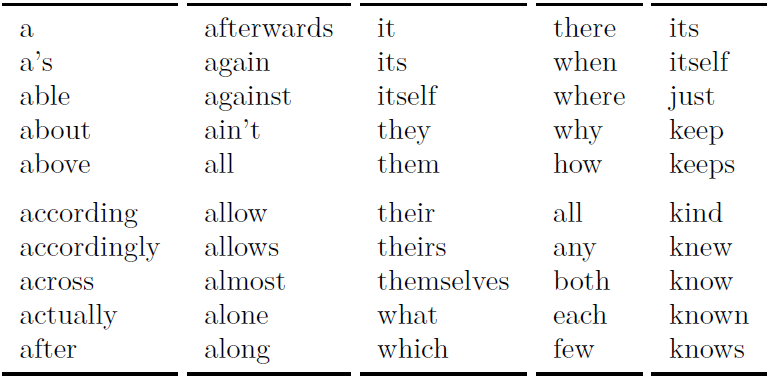
\includegraphics[scale = 0.50]{figuras/stopwords.PNG}
	\fonte{Elaboração do autor.}
\end{table}

Para cada documento de corpo textual das atas do Copom, foi aplicado o processo de \textit{stopwords} (remoção de palavras comuns), provenientes de uma compilação presente no pacote \textit{tidytext} reunido por \citeonline{silge2016tidytext}, que contém 1149 palavras de três diferentes dicionários léxicos: \textit{SMART}, \textit{snowball} e \textit{onix}. Para fins de exemplificação, algumas dessas \textit{stopwords} podem ser observadas na Tabela \ref{table:stopwords}.

Não obstante, palavras adicionais que para a análise desta pesquisa julgou-se irrelevante foram desconsideradas, tais quais meses do ano (como \textit{'january'}, \textit{'month'}, \textit{'monthly'}), nomes próprios (como \textit{'aloisio'}, \textit{'guardado'}, \textit{'rumenos'}), numerais (como \textit{'one'}, \textit{'two'}, \textit{'three'}). Também desconsiderou-se palavras com erros de interpretação devido a quebras de linha (como \textit{'nmonetary'}, \textit{'nexecutive'}, \textit{'npandemic'}).

\subsection{Variáveis macroeconômicas}

Os dados macroeconômicos utilizados para comparação do índice de sentimentos foram reunidos do BCB e do Instituto Brasileiro de Geografia e Estatística (IBGE).

Conforme inicialmente propõe \citeonline{bloom2009uncertainty} e posteriormente \citeonline{ferreira2017incerteza} para o Brasil, baseando-se nesses estudos e considerando algumas alterações, o trabalho englobou as seguintes variáveis:

\begin{enumerate}[noitemsep,nosep,labelindent=\parindent,leftmargin=*,label={\alph*}) ] 
	\item para representar a taxa básica de juros da economia brasileira, usou-se taxa Selic Meta, definida nas reuniões do Copom a cada quarenta e cinco dias;
	\item para a medida de inflação, o Índice Nacional de Preços ao Consumidor Amplo (IPCA), que contempla uma cesta de bens e serviços referentes ao consumo pessoal das famílias de um até quarenta salários mínimos das principais regiões metropolitanas do país;
	\item para a atividade econômica, usou-se do Índice de Atividade Econômica do Banco Central (IBC-Br), que serve como indicador agregado de atividade econômica com frequência mensal;
	\item para representar a produção industrial, utilizou-se a Pesquisa Industrial Mensal de Produção Física (PIM-PF)
\end{enumerate}

A relação resumida das variáveis, sua descrição, seu código nas bases de dados oficiais e sua fonte podem ser observadas na Tabela \ref{table:variaveis_metodologia}:

\begin{table}[hbtp]
	\centering
	\caption{Resumo das variáveis macroeconômicas} \label{table:variaveis_metodologia}
	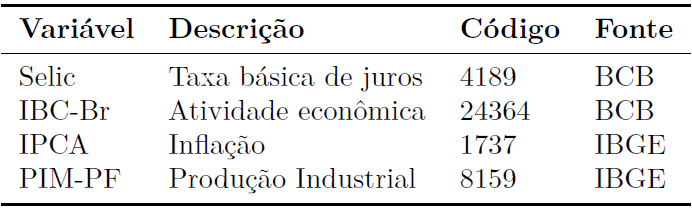
\includegraphics[scale = 0.50]{figuras/variaveis_metodologia.PNG}
	\fonte{Elaboração do autor.}
\end{table}

Os dados de taxa de juros e atividade econômica foram obtidos pelo do Sistema Gerenciador de Séries Temporais (SGS) do BCB, sendo a de código 4189 a taxa de juros Selic acumulada no mês, anualizada base 252, como \%a.a., com periodicidade mensal; e a de código 24364 o "Índice de Atividade Econômica do Banco Central (IBC-Br), aplicado ajuste sazonal, com periodicidade mensal. 

Os dados de inflação e produção industrial foram adquiridos do Sistema IBGE de Recuperação Automática (SIDRA), com código 1737 e 8159, respectivamente.

Como a taxa básica de juros estava anualizada com periodicidade mensal, transformou-se ela em mensal e acumulou-se em número-índice. Da inflação e da taxa básica de juros então calculou-se o valor acumulado em doze meses, de acordo:

\begin{ceqn}
\begin{align} \label{}
\textit{Índice}_{12m, t} = \frac{\textit{Índice}_{t}}{\textit{Índice}_{t-12}} - 1 
\end{align}
\end{ceqn} em que o $\textit{Índice}_{t}$ é o valor do Índice no tempo $t$; o $\textit{Índice}_{t-12}$ é o valor do Índice doze meses após $t$; e $\textit{Índice}_{12m, t}$ é o Índice acumulado no tempo $t$. Com isso, foi possível obter a série da taxa de juros real, descontando a inflação da taxa básica de juros.

Para as séries da inflação e taxa básica de juros haviam-se dados até maio de 2022; para a série da produção industrial até abril de 2022 e para a série de atividade econômica até fevereiro de 2022. Dessa maneira, optou-se por trabalhar com dados até fevereiro de 2022.